\section{Data and Methods}
\label{sec:data}

[SECTION TO BE EXPANDED BY OPUS]

% When filled in:
% - Dataset description
% - Sample characteristics
% - Calibration metrics (MAE, Brier)
% - Statistical inference

\subsection{Dataset: Kalshi Prediction Markets}
\label{subsec:dataset}

% Sample composition table with TikZ chart

\subsubsection{Sample Characteristics}

\begin{figure}[h]
\centering
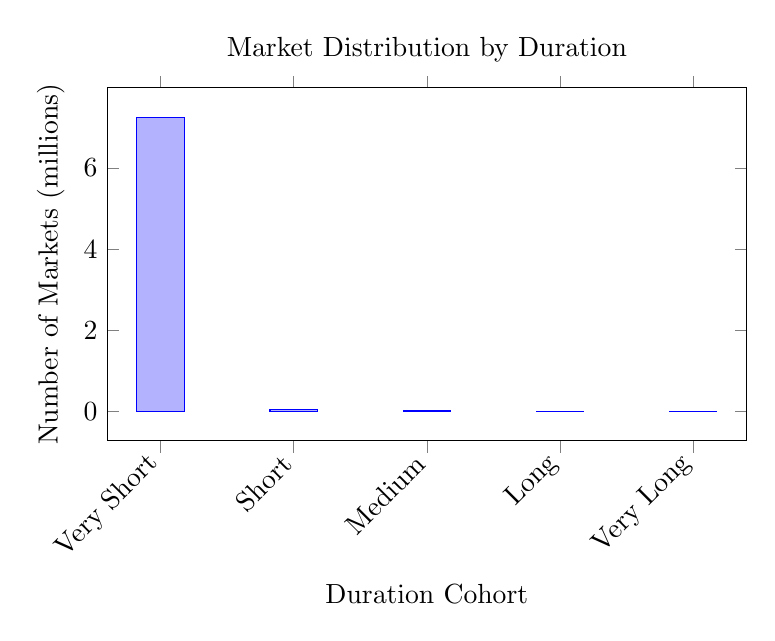
\begin{tikzpicture}
  \begin{axis}[
    title={Market Distribution by Duration},
    xlabel={Duration Cohort},
    ylabel={Number of Markets (millions)},
    ybar,
    bar width=0.6cm,
    width=0.8\textwidth,
    height=0.5\textwidth,
    xtick={1,2,3,4,5},
    xticklabels={Very Short, Short, Medium, Long, Very Long},
    x tick label style={rotate=45, anchor=east}
  ]
    % Data from Table 1 (line numbers from markdown)
    \addplot coordinates {(1, 7.25) (2, 0.05) (3, 0.01) (4, 0.006) (5, 0.0004)};
  \end{axis}
\end{tikzpicture}
\caption{Distribution of analyzed markets by duration. Note: 99.2\% of Kalshi markets resolve within 7 days.}
\label{fig:sample_dist}
\end{figure}

\subsection{Calibration Metrics}
\label{subsec:metrics}

% MAE and Brier score formulas and definitions

\subsection{Statistical Inference}
\label{subsec:inference}

% CI computation, hypothesis tests, etc.
